\documentclass[11pt]{exam}
\usepackage[margin=1in]{geometry}
\usepackage{amsfonts, amsmath, amssymb, amsthm}
\usepackage{mathtools}
\usepackage{enumerate}
\usepackage{listings}
\usepackage{colortbl}
\usepackage{float}
\usepackage[colorlinks,linkcolor=blue]{hyperref}

% in order to compile this file you need to get 'header.tex' from
% Canvas and change the line below to the appropriate file path
%%% theorems

\theoremstyle{plain}            % following are "theorem" style
\newtheorem{theorem}{Theorem}[section]
\newtheorem{lemma}[theorem]{Lemma}
\newtheorem{corollary}[theorem]{Corollary}
\newtheorem{proposition}[theorem]{Proposition}
\newtheorem{claim}[theorem]{Claim}
\newtheorem{fact}[theorem]{Fact}
\newtheorem{openproblem}[theorem]{Open Problem}

\theoremstyle{definition}       % following are def style
\newtheorem{definition}[theorem]{Definition}
\newtheorem{conjecture}[theorem]{Conjecture}
\newtheorem{example}[theorem]{Example}
\newtheorem{protocol}[theorem]{Protocol}
\newtheorem{exercise}[theorem]{Exercise}

\theoremstyle{remark}           % following are remark style
\newtheorem{remark}[theorem]{Remark}
\newtheorem{note}[theorem]{Note}
%\newtheorem*{solution}{Solution}

%%% special sets
\newcommand{\bit}{\ensuremath{\{0,1\}}}
\newcommand{\bitt}{\ensuremath{\{-1,1\}}}
\newcommand{\ball}{\ensuremath{\mathcal{B}}}
\newcommand{\sph}{\ensuremath{\mathbb{S}}}
\newcommand{\odisc}[2]{\ensuremath{D(#1, #2)}}
\newcommand{\cdisc}[2]{\ensuremath{\bar{D}(#1, #2)}}
\newcommand{\emp}{\varnothing}

% constants
\newcommand{\E}{\ensuremath{\mathrm{e}}}
\newcommand{\I}{\ensuremath{\mathrm{i}}}
\newcommand{\Id}{\ensuremath{\mathrm{I}}}
\newcommand{\paulix}{\ensuremath{\mathrm{X}}}
\newcommand{\pauliy}{\ensuremath{\mathrm{Y}}}
\newcommand{\pauliz}{\ensuremath{\mathrm{Z}}}

% font for general-purpose algorithms
\newcommand{\algo}[1]{\ensuremath{\mathsf{#1}}}
% font for general-purpose computational problems
\newcommand{\problem}[1]{\ensuremath{\mathsf{#1}}}
% font for complexity classes
\newcommand{\class}[1]{\ensuremath{\mathsf{#1}}}

% asymptotics
\DeclareMathOperator{\poly}{poly}
\DeclareMathOperator{\polylog}{polylog}
\DeclareMathOperator{\negl}{negl}
\DeclareMathOperator{\bigO}{O}
\DeclareMathOperator{\litO}{o}
\DeclareMathOperator{\Otil}{\tilde{O}}
\DeclareMathOperator{\Ostar}{O^*}

%%% "LEFT-RIGHT" PAIRS OF SYMBOLS

% inner product
\DeclarePairedDelimiter\inner{\langle}{\rangle}
% absolute value
\DeclarePairedDelimiter\abs{\lvert}{\rvert}
% a set
\DeclarePairedDelimiter\set{\{}{\}}
% parens
\DeclarePairedDelimiter\parens{(}{)}
% tuple, alias for parens
\DeclarePairedDelimiter\tuple{(}{)}
% square brackets
\DeclarePairedDelimiter\bracks{[}{]}
% rounding off
\DeclarePairedDelimiter\round{\lfloor}{\rceil}
% floor function
\DeclarePairedDelimiter\floor{\lfloor}{\rfloor}
% ceiling function
\DeclarePairedDelimiter\ceil{\lceil}{\rceil}
% length of some vector, element
\DeclarePairedDelimiter\length{\lVert}{\rVert}
% "lifting" of a residue class
\DeclarePairedDelimiter\lift{\llbracket}{\rrbracket}
\DeclarePairedDelimiter\len{\lvert}{\rvert}
% bra-kets
\DeclarePairedDelimiter\bra{\langle}{\rvert}
\DeclarePairedDelimiter\ket{\lvert}{\rangle}
\newcommand{\braket}[2]{\ensuremath{\langle #1 \vert #2 \rangle}}
\newcommand{\ketbra}[2]{\ensuremath{\lvert #1 \rangle \langle #2 \rvert}}

%%% spacing

\newcommand{\ws}{\hspace{1pt}}
\newcommand{\wws}{\hspace{2pt}}
\newcommand{\hs}{\hspace{4pt}}
\newcommand{\hhs}{\hspace{8pt}}
\newcommand{\hhhs}{\hspace{12pt}}

%%% LISTS

\newcommand{\oneto}{1, \ldots,}
\newcommand{\onetop}{1 \cdots,}
\newcommand{\zeroto}{0, \ldots,}
\newcommand{\zerotop}{0 \cdots,}
\newcommand{\perm}[1]{\mathbf{(#1)}}
\newcommand{\permv}[1]{(#1)}
\newcommand{\varind}[2]{#1_1, \ldots, #1_#2}
\newcommand{\varindz}[2]{#1_0, \ldots, #1_#2}
\newcommand{\varindp}[2]{#1_1 \cdots #1_#2}
\newcommand{\varindpz}[2]{#1_0 \cdots #1_#2}
\newcommand{\seq}[2]{(#1_#2)_{#2=1}^\infty}
\newcommand{\seqz}[2]{(#1_#2)_{#2=0}^\infty}

%%% MATH OPERATORS

%\DeclareMathOperator{\pr}{\mathbf{P}}
%\DeclareMathOperator{\ex}{\mathbf{E}}
\DeclareMathOperator{\pr}{P}
\DeclareMathOperator{\ex}{E}
\DeclareMathOperator{\Span}{Span}
\DeclareMathOperator{\tr}{Tr}
\DeclareMathOperator{\supp}{Supp}
\DeclareMathOperator{\im}{Im}
\DeclareMathOperator{\var}{var}
\DeclareMathOperator{\vol}{vol}
\DeclareMathOperator{\sign}{sign}
\DeclareMathOperator{\dkl}{D_{KL}}
\DeclareMathOperator{\entr}{H}
\DeclareMathOperator{\fid}{F}
\DeclareMathOperator{\dist}{D}
\DeclareMathOperator{\ad}{ad}

% hats

\newcommand{\fhat}{\ensuremath{\hat{f}}}
\newcommand{\phat}{\ensuremath{\hat{p}}}
\newcommand{\that}{\ensuremath{\hat{t}}}

%%% BLACKBOARD SYMBOLS

% \newcommand{\C}{\ensuremath{\mathbb{C}}}
\newcommand{\D}{\ensuremath{\mathbb{D}}}
\newcommand{\F}{\ensuremath{\mathbb{F}}}
% \newcommand{\G}{\ensuremath{\mathbb{G}}}
\newcommand{\J}{\ensuremath{\mathbb{J}}}
\newcommand{\N}{\ensuremath{\mathbb{N}}}
\newcommand{\Q}{\ensuremath{\mathbb{Q}}}
\newcommand{\R}{\ensuremath{\mathbb{R}}}
\newcommand{\T}{\ensuremath{\mathbb{T}}}
\newcommand{\Z}{\ensuremath{\mathbb{Z}}}
\newcommand{\QR}{\ensuremath{\mathbb{QR}}}

% sets in calligraphic type

\newcommand{\calD}{\ensuremath{\mathcal{D}}}
\newcommand{\calF}{\ensuremath{\mathcal{F}}}
\newcommand{\calG}{\ensuremath{\mathcal{G}}}
\newcommand{\calH}{\ensuremath{\mathcal{H}}}
\newcommand{\calI}{\ensuremath{\mathcal{I}}}
\newcommand{\calL}{\ensuremath{\mathcal{L}}}
\newcommand{\calN}{\ensuremath{\mathcal{N}}}
\newcommand{\calP}{\ensuremath{\mathcal{P}}}
\newcommand{\calS}{\ensuremath{\mathcal{S}}}
\newcommand{\calX}{\ensuremath{\mathcal{X}}}
\newcommand{\calY}{\ensuremath{\mathcal{Y}}}

% matrices and vectors

\newcommand{\matA}{\ensuremath{\mathbf{A}}}
\newcommand{\matB}{\ensuremath{\mathbf{B}}}
\newcommand{\matC}{\ensuremath{\mathbf{C}}}
\newcommand{\matD}{\ensuremath{\mathbf{D}}}
\newcommand{\matE}{\ensuremath{\mathbf{E}}}
\newcommand{\matF}{\ensuremath{\mathbf{F}}}
\newcommand{\matG}{\ensuremath{\mathbf{G}}}
\newcommand{\matH}{\ensuremath{\mathbf{H}}}
\newcommand{\matI}{\ensuremath{\mathbf{I}}}
\newcommand{\matJ}{\ensuremath{\mathbf{J}}}
\newcommand{\matK}{\ensuremath{\mathbf{K}}}
\newcommand{\matL}{\ensuremath{\mathbf{L}}}
\newcommand{\matM}{\ensuremath{\mathbf{M}}}
\newcommand{\matN}{\ensuremath{\mathbf{N}}}
\newcommand{\matO}{\ensuremath{\mathbf{O}}}
\newcommand{\matP}{\ensuremath{\mathbf{P}}}
\newcommand{\matQ}{\ensuremath{\mathbf{Q}}}
\newcommand{\matR}{\ensuremath{\mathbf{R}}}
\newcommand{\matS}{\ensuremath{\mathbf{S}}}
\newcommand{\matT}{\ensuremath{\mathbf{T}}}
\newcommand{\matU}{\ensuremath{\mathbf{U}}}
\newcommand{\matV}{\ensuremath{\mathbf{V}}}
\newcommand{\matW}{\ensuremath{\mathbf{W}}}
\newcommand{\matX}{\ensuremath{\mathbf{X}}}
\newcommand{\matY}{\ensuremath{\mathbf{Y}}}
\newcommand{\matZ}{\ensuremath{\mathbf{Z}}}
\newcommand{\matzero}{\ensuremath{\mathbf{0}}}

\newcommand{\veca}{\ensuremath{\mathbf{a}}}
\newcommand{\vecb}{\ensuremath{\mathbf{b}}}
\newcommand{\vecc}{\ensuremath{\mathbf{c}}}
\newcommand{\vecd}{\ensuremath{\mathbf{d}}}
\newcommand{\vece}{\ensuremath{\mathbf{e}}}
\newcommand{\vecf}{\ensuremath{\mathbf{f}}}
\newcommand{\vecg}{\ensuremath{\mathbf{g}}}
\newcommand{\vech}{\ensuremath{\mathbf{h}}}
\newcommand{\veck}{\ensuremath{\mathbf{k}}}
\newcommand{\vecm}{\ensuremath{\mathbf{m}}}
\newcommand{\vecp}{\ensuremath{\mathbf{p}}}
\newcommand{\vecq}{\ensuremath{\mathbf{q}}}
\newcommand{\vecr}{\ensuremath{\mathbf{r}}}
\newcommand{\vecs}{\ensuremath{\mathbf{s}}}
\newcommand{\vect}{\ensuremath{\mathbf{t}}}
\newcommand{\vecu}{\ensuremath{\mathbf{u}}}
\newcommand{\vecv}{\ensuremath{\mathbf{v}}}
\newcommand{\vecw}{\ensuremath{\mathbf{w}}}
\newcommand{\vecx}{\ensuremath{\mathbf{x}}}
\newcommand{\vecy}{\ensuremath{\mathbf{y}}}
\newcommand{\vecz}{\ensuremath{\mathbf{z}}}
\newcommand{\veczero}{\ensuremath{\mathbf{0}}}
\newcommand{\vecone}{\ensuremath{\mathbf{1}}}

\newcommand{\vecell}{\ensuremath{\boldsymbol\ell}}
\newcommand{\vecalpha}{\ensuremath{\boldsymbol\alpha}}
\newcommand{\vecbeta}{\ensuremath{\boldsymbol\beta}}
\newcommand{\veceta}{\ensuremath{\boldsymbol\eta}}
\newcommand{\vecmu}{\ensuremath{\boldsymbol\mu}}
\newcommand{\vecphi}{\ensuremath{\boldsymbol\phi}}
\newcommand{\vecsigma}{\ensuremath{\boldsymbol\sigma}}
\newcommand{\vectheta}{\ensuremath{\boldsymbol\theta}}
\newcommand{\vecxi}{\ensuremath{\boldsymbol\xi}}

%%% misc

\newcommand{\ind}{\ensuremath{\mathbf{1}}}

\newcommand{\congmod}[3]{#1 \equiv #2 \textrm{ modulo } #3}

\newcommand{\dee}{\,\mathrm{d}}
\newcommand{\de}{\mathrm{d}}
\newcommand{\dx}{\,\mathrm{d} x}

\newcommand{\ol}{\overline}
\newcommand{\inv}[1]{\ensuremath{#1^{-1}}}
\newcommand{\tsp}[1]{\ensuremath{#1^{\top}}}


\newcommand{\eps}{\varepsilon}
\newcommand{\ph}{\varphi}

\newcommand{\Ra}{\Rightarrow}
\newcommand{\Lra}{\Leftrightarrow}
\newcommand{\rsqa}{\rightsquigarrow}

\newcommand{\trl}{\triangleleft}
\newcommand{\trr}{\triangleright}

\newcommand{\func}[3]{#1: #2 \to #3}
\newcommand{\dd}[1]{\frac{\mathrm{d}}{\mathrm{d}#1}}
\newcommand{\ptl}[1]{\frac{\partial}{\partial #1}}
\newcommand{\prtl}[2]{\frac{\partial #1}{\partial #2}}

\newcommand{\matrixtt}[4]{
  \begin{pmatrix*}[r]
        #1 & #2 \\
        #3 & #4
    \end{pmatrix*}
}

%%% for homework and section notes

\newcommand{\commonheader}[2]{
    \pagestyle{headandfoot}
    \setlength{\headheight}{26pt}
    \setlength{\headsep}{30pt}

    \header
        {\small{\textbf{VE281: Data Structures and Algorithms}} \\ \footnotesize{\textbf{UM-SJTU Joint Institute, FA2021}}}
        {#1}
        {#2}

    \firstpageheadrule
    \runningheadrule

    \footer
        {}
        {\thepage}
        {}
}

\newcommand{\hwheader}{
    \commonheader
        {\textbf{Homework \hwnum}}
        {\small \textbf{Due at \duedate}}
}

\newcommand{\hwslnheader}{
    \commonheader
    	{}
        {\textbf{Solutions to Homework \hwnum}}
    \printanswers
}

\newcommand{\notesheader}{
    \commonheader
        {\Large \textbf{Section Notes \sectionnum}}
    	{}
}

\newcommand{\hint}[1]{
\emph{Hint}: #1
}

% for effort questions
\let\Eitem=\relax
\def\effortE{\textbf{E}~}
\makeatletter
\def\Eitem{%
    \expandafter\let\expandafter\originallabel\csname labelenum\romannumeral\@enumdepth\endcsname
    \expandafter\def\csname labelenum\romannumeral\@enumdepth\expandafter\endcsname\expandafter{%
        \expandafter\effortE\originallabel}%
    \item
    \expandafter\let\csname labelenum\romannumeral\@enumdepth\endcsname\originallabel
}
\makeatother

\allowdisplaybreaks


\geometry{left=2.5 cm,right=2.5 cm,top=2.5 cm,bottom=2.5 cm}
%\pagestyle{fancy}
\definecolor{mygreen}{rgb}{0,0.6,0}  
\definecolor{mygray}{rgb}{0.5,0.5,0.5}
\definecolor{mymauve}{rgb}{0.58,0,0.82} 
\definecolor{background}{rgb}{0.963,0.963,0.963}

\definecolor{codegreen}{rgb}{0,0.6,0}
\definecolor{codegray}{rgb}{0.5,0.5,0.5}
\definecolor{codepurple}{rgb}{0.58,0,0.82}
\definecolor{backcolour}{rgb}{0.95,0.95,0.92}

\lstdefinestyle{mystyle}{
    backgroundcolor=\color{backcolour},   
    commentstyle=\color{codegreen},
    keywordstyle=\color{magenta},
    numberstyle=\tiny\color{codegray},
    stringstyle=\color{codepurple},
    basicstyle=\ttfamily\footnotesize,
    breakatwhitespace=false,         
    breaklines=true,                 
    captionpos=b,                    
    keepspaces=true,                 
    numbers=left,                    
    numbersep=5pt,                  
    showspaces=false,                
    showstringspaces=false,
    showtabs=false,                  
    tabsize=2
}

\lstset{style=mystyle}
\newcommand{\hwnum}{3}
\newcommand{\duedate}{11:59pm, November 9th}

%\notesheader
\hwheader   % header for homework
%\hwslnheader   % header for homework solutions

% Comment the following line in order to hide solutions.
% Uncomment the line to show solutions written inside of
% LaTeX solution environments like:
%   \begin{solution}
%     My solution.
%   \end{solution}.
\printanswers

\begin{document}
\setlength{\parindent}{0pt}
\section*{Before you start:}

\subsection*{Homework Files}
You can download the starter files for coding as well as this \textit{tex} file (you only need to modify \textit{homework3.tex}) on canvas and do your homework with latex. Or you can scan your handwriting, convert to pdf file, and upload it to canvas before the due date. If you choose to write down your answers by hand, you can directly download the pdf file on canvas which provides more blank space for solution box.\\

\subsection*{Submission Form}
For homework 3, there are only one part of submission, which is a pdf file as your solution named as VE281\_HW3\_[Your Student ID]\_[Your name].pdf uploaded to canvas.

Estimated time used for this homework: \textbf{3-4 hours.}
\\\\
Great credits to 2020FA VE281 TA Group and enormous thanks to 2021SU VE281 TA Roihn!!!

\newpage
\section*{0\quad Student Info (0 point)}
Your name and student id:
\begin{solution}
% Write your answer here
\end{solution}

\section{Tree Traversal (27 points)}

\subsection{Given A Tree (16 points)}
Given a binary tree below, please write out the following traversals:
\begin{figure}[H]
\centering
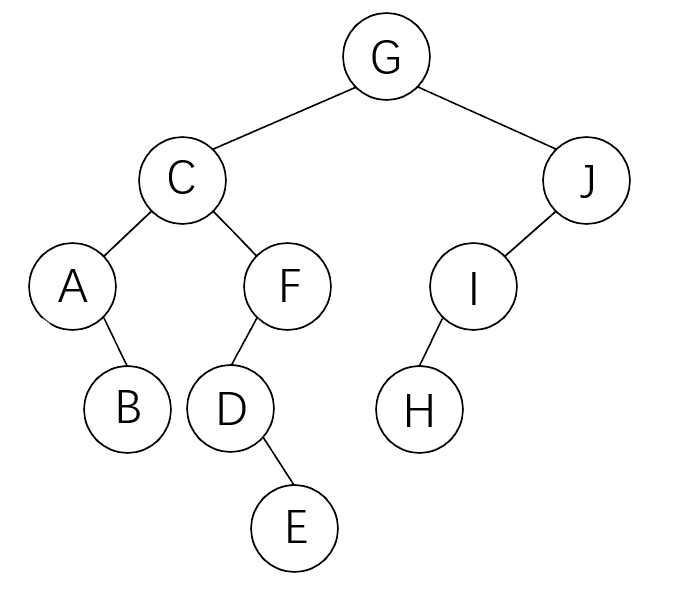
\includegraphics[width=.5\linewidth]{binary_tree.png}
\end{figure}
\begin{enumerate}[(a)]
\item Pre-order depth-first traversal. (4 points)
\begin{solution}
%Write your answer here.
\end{solution}

\item Post-order depth-first traversal. (4 points)
\begin{solution}
%Write your answer here.
\end{solution}

\item In-order depth-first traversal. (4 points)
\begin{solution}
%Write your answer here.
\end{solution}

\item Level-order traversal. (4 points)
\begin{solution}
%Write your answer here.
\end{solution}

\end{enumerate}


\subsection{Draw The Tree (11 points)}
\begin{enumerate}[a)]
\item Now we have a specific binary tree, but we only know some of its traversals. Its pre-order traversal is: \textbf{FBADCEGIH}, and its in-order traversal is: \textbf{ABCDEFGHI}. Then please \textbf{draw out the binary tree} and show its \textbf{post-order traversal}. (4 points)

\begin{solution}
%Write your answer here.
\end{solution}

\item Now we have a specific binary tree, but we only know some of its traversals. Its post-order traversal is: \textbf{FEKLJIHG}, and its in-order traversal is: \textbf{EFGHIKJL}. Then please \textbf{draw out the binary tree} and show its \textbf{pre-order traversal}. (4 points)

\begin{solution}
%Write your answer here.
\end{solution}

\item Now students are required to draw out the binary tree according to the given traversals: Its pre-order traversal is: \textbf{ACDFGEB}, and its post-order traversal is: \textbf{DCEBGFA}. Then please \textbf{draw out the binary tree} and show its \textbf{pre-order traversal}.

William and Coned both provide their plot of the unknown trees. 
\begin{figure}[H]
\centering
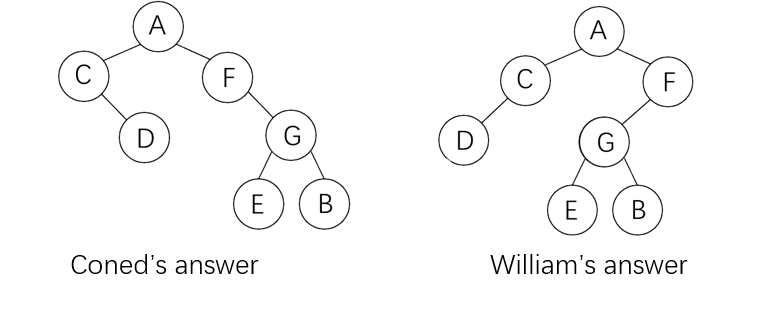
\includegraphics[width=.8\linewidth]{Coned_vs_William.png}
\end{figure}

Their answers are totally different, but seem to be both correct. Can you explain why such a case happens? (3 points)

\begin{solution}
%Write your answer here.
\end{solution}

\end{enumerate}


\section{True or False (20 points)}
Please judge whether the following statements are \textbf{TRUE} or \textbf{FALSE}. You can briefly state your reason if you would like to get partial points. No deduction if the solution is right without explanation. Each question takes 2 points.
	\begin{enumerate}[a)]
		\item A complete tree is a tree where every node has either 0 or 2 children.
		\begin{solution}
%Write your answer here.
\end{solution}
		\item A complete tree is a tree where every level except the last is necessarily filled, and in the last level, nodes are filled in from left to right.
\begin{solution}
%Write your answer here.
\end{solution}
		\item Heapsort has worst-case $\Theta(n \log n)$ time complexity.
		\begin{solution}
%Write your answer here.
\end{solution}
		\item  Percolate-up has an average-case time complexity of $\Theta(\log n)$.
\begin{solution}
%Write your answer here.
\end{solution}
		\item Dequeue is done by simply removing the root.
\begin{solution}
%Write your answer here.
\end{solution}
		\item Enqueue in a min-heap is done by inserting the element at the end, and then calling percolate-up.
\begin{solution}
%Write your answer here.
\end{solution}
		\item $[1, 13, 17, 23, 14, 16, 20, 35]$ is a representation of a min-heap.
\begin{solution}
%Write your answer here.
\end{solution}
		\item $[83, 47, 9, 22, 15, 7, 1, 20]$ is a representation of a \textbf{max-heap}.
\begin{solution}
%Write your answer here.
\end{solution}
		\item  Proceeding from the bottom of the heap to the top, while repeatedly calling percolateDown() can initialize a min-heap.
\begin{solution}
%Write your answer here.
\end{solution}
		\item Proceeding from the top of the heap to the bottom, while repeatedly calling percolateUp() can not initialize a min-heap.
		\begin{solution}
%Write your answer here.
\end{solution}
	\end{enumerate}

\section{Min Heap (23 points)}
Consider a min-heap represented by the following array:
\begin{align*}
\{2, 3, 8, 16, 46, 34, 42, 35, 26\}
\end{align*}

Perform the following operations using the algorithms for binary heaps discussed in lecture. Ensure that the heap property is restored at the end of every individual operation.

For the following operations, tell how many percolations(either up or down) are needed and show the result of the heap after each \textbf{percolation} in either tree form or array form. 

\begin{enumerate}[a)]
\item Push the value of 1 into this min-heap. (4 points)
\begin{solution}
%Write your answer here.
\end{solution}

\item After a), push the value of 5 into this min-heap. (4 points)
\begin{solution}
%Write your answer here.
\end{solution}

\item After b), update element 2 to have a value of 37 (Suppose you have the access to each element). (5 points)
\begin{solution}
%Write your answer here.
\end{solution}

\item After c), remove the min element from the heap. (5 points)
\begin{solution}
%Write your answer here.
\end{solution}

\item After d), update element 26 to have a value of 4 (Suppose you have the access to each element) (5 points)
\begin{solution}
%Write your answer here.
\end{solution}

\end{enumerate}

\section{Binary Search Tree (30 points)}
\subsection{Simple simulation (16 points)}

Perform the following operations to construct a binary search tree. Show the result of the BST after each operation in either tree form or array form.

\begin{enumerate}[a)]
\item Insert 24, 29, 22, 25, 19, 32, 15, 37 (3 points)
\begin{solution}
%Write your answer here.
\end{solution}

\item Delete 22 (3 points)
\begin{solution}
%Write your answer here.
\end{solution}

\item Delete 29 (3 points)
\begin{solution}
%Write your answer here.
\end{solution}

\item Insert 22 (3 points)
\begin{solution}
%Write your answer here.
\end{solution}

\item What is the in-order predecessor of node 25? What is the in-order successor of node 32? (4 points)
\begin{solution}
%Write your answer here.
\end{solution}


\end{enumerate}

\subsection{Better than linear selection? (14 points)}
After learning the application of the BST, Coned thinks that with BST, rank search can be done either in a faster way or with less space compared with the linear selection algorithms introduced in the lecture.
\begin{enumerate}[a)]
    \item Compare BST rank search with deterministic selection algorithm in terms of time complexity and space usage. Assume that for each node, a variable \textit{leftsize} is maintained as introduced in the lecture. (8 points)
    \begin{solution}
    %Write your answer here.
    \end{solution}
    \item William, our master of algorithm, has a different idea again. He states that for the linear selection algorithm, the input can be arbitrary array while for BST rank search, you have to first build up a binary search tree from the arbitrary array, which will also take some time. Therefore, the average time complexity of BST rank search is not better than $O(n)$. Is he right? (6 points)\\
    Assume that we are working on a fixed array and doing lots of rank search.
    \begin{solution}
    %Write your answer here.
    \end{solution}
\end{enumerate}

\section*{Reference}
Assignment 3, VE281, FA2020, UMJI-SJTU.

Homework 2, VE281, SU2021, UMJI-SJTU.

\end{document}